\documentclass[12pt,a4paper]{article}
\usepackage[utf8]{inputenc}
\usepackage[english]{babel}
\usepackage{amsmath}
\usepackage{amsfonts}
\usepackage{amssymb}
\usepackage{graphicx}
\usepackage[left=2.5cm,right=2.5cm,top=2.5cm,bottom=2.5cm]{geometry}
\usepackage{setspace}
\usepackage{cite}
\usepackage{url}
\usepackage{enumitem}
\usepackage{float}
\usepackage{placeins}

\title{Report on the Impact and Bioinformatics of Alternative Splicing}
\author{Samuel J. Koch \\
        Technical University of Munich (TUM) \\
        Problem Based Learning Bioinformatics (PBL) \\
        Supervisor: Prof. Dr. rer. nat. Dimitri Frischmann \\
        Summer Semester 2025}
\date{June 24, 2025}

\begin{document}

\maketitle
\newpage

\tableofcontents
\newpage

\doublespacing

\begin{abstract}
Alternative splicing (AS) is a fundamental biological process that enables a single gene to produce multiple protein isoforms, significantly contributing to proteomic diversity in eukaryotic organisms. This report examines two influential studies: Liu et al. (2017) ``Impact of Alternative Splicing on the Human Proteome'', which developed an integrative experimental approach combining RNA-seq with mass spectrometry to quantitatively assess how splicing perturbations affect proteome composition, and Florea (2005) ``Bioinformatics of alternative splicing and its regulation'', which provides a comprehensive overview of bioinformatics methods for identifying and characterizing alternative splicing events and their regulatory elements. The integrative approach successfully demonstrated that changes in mRNA splicing patterns translate into measurable protein abundance changes, with intron retention consistently associated with decreased protein levels and differential transcript usage producing proportionate protein changes. Bioinformatics methods ranging from sequence comparison to splice graph modeling have proven effective for cataloguing splicing variants, though challenges remain in distinguishing biologically relevant isoforms from computational artifacts. These advances establish a foundation for therapeutic interventions targeting splicing defects in human diseases and open new possibilities for personalized medicine approaches based on isoform signatures.
\end{abstract}

\newpage

\section{Introduction}

Alternative splicing (AS) represents one of the most important mechanisms by which eukaryotic organisms achieve biological complexity from a relatively limited genetic repertoire. This process allows a single gene to produce multiple messenger RNA (mRNA) and protein isoforms by selectively combining different exons during RNA processing. The significance of alternative splicing becomes apparent when considering that humans possess only approximately 25,000 protein-coding genes ([3]), yet produce hundreds of thousands of distinct proteins with diverse functions, localizations, and regulatory properties.

\begin{figure}[H]
\centering
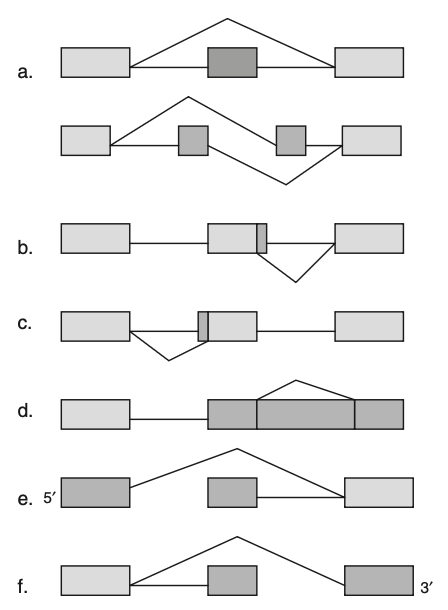
\includegraphics[width=0.6\textwidth]{alt_splicing_figure_1_florea.png}
\caption{Types of alternative splicing events: (a) exon inclusion/exclusion; (b) alternative 3' end; (c) alternative 5' end; (d) intron retention; (e,f) alternative UTRs. Adapted from Florea (2005).}
\label{fig:alt_splicing_types}
\end{figure}

The molecular mechanism of alternative splicing involves the selective inclusion or exclusion of exons during the maturation of pre-mRNA transcripts. Different combinations of exons can be incorporated into the final mRNA molecule, with each unique transcript serving as a template for producing distinct protein variants. These protein isoforms may exhibit dramatically different, and sometimes antagonistic, functional and structural properties, enabling fine-tuned regulation of cellular processes across different tissues, developmental stages, and environmental conditions.

The biological importance of alternative splicing extends far beyond simply increasing protein diversity. Defects in mRNA splicing patterns and their regulation have been implicated in numerous human diseases, including various cancers, neurological disorders, and genetic diseases. Understanding how splicing perturbations affect protein abundance and function is therefore crucial for developing therapeutic strategies and diagnostic approaches.

Despite decades of research, a major challenge has been quantitatively linking the well-documented transcriptomic diversity generated by alternative splicing to its actual impact on the proteome. While RNA sequencing has revealed extensive splicing variation, the functional consequences at the protein level have remained largely unmeasured. This gap between transcriptomic and proteomic understanding has limited our ability to predict the biological significance of observed splicing changes and to develop targeted therapeutic interventions.

This report examines two complementary approaches to understanding alternative splicing: the experimental quantification of splicing impact on protein abundance, and the bioinformatics methods developed to identify and characterize splicing events and their regulation. The motivation for this analysis is to evaluate how these methodological advances have enhanced our understanding of alternative splicing and to assess their potential for future therapeutic applications.

\section{Approach}

\subsection{Integrative Experimental Methods}

Liu et al. (2017) developed a comprehensive experimental framework to quantitatively assess the impact of alternative splicing perturbations on proteome composition ([1], p. 1229). Their approach represents a significant methodological advance by directly linking transcriptomic changes to proteomic outcomes.

\begin{figure}[H]
\centering
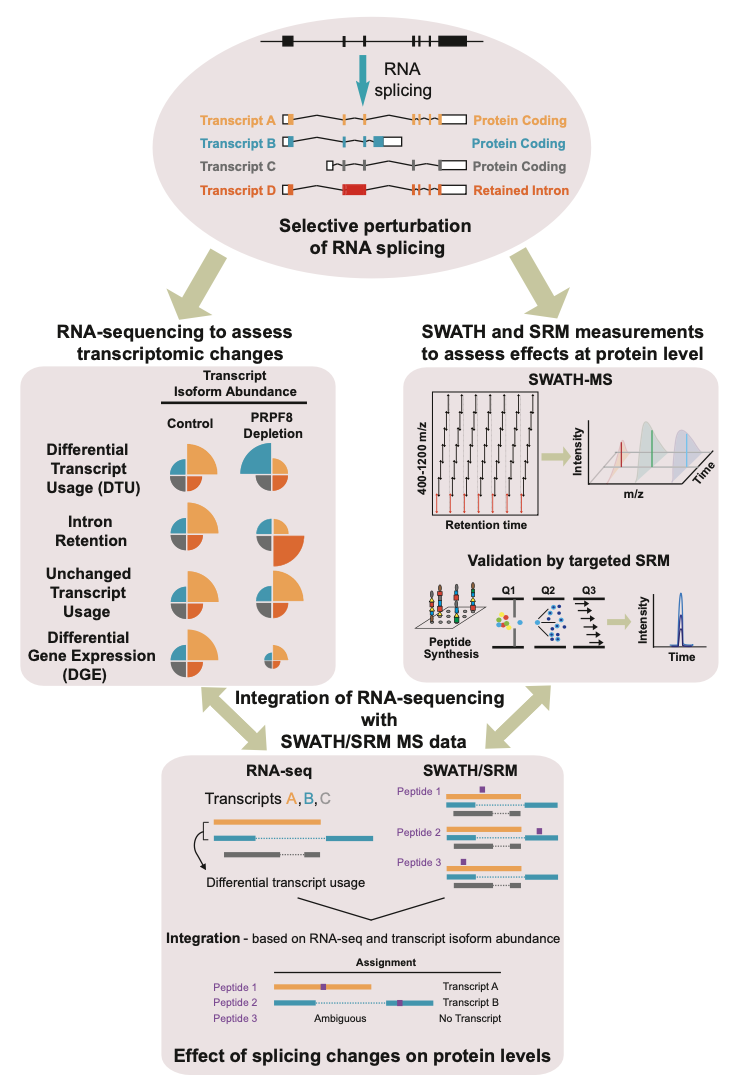
\includegraphics[width=0.6\textwidth]{framework_figure_1_liu.png}
\caption{Experimental framework integrating RNA-seq and mass spectrometry to study alternative splicing impact on the proteome. Adapted from Liu et al. (2017).}
\label{fig:experimental_framework}
\end{figure}

\subsubsection{Experimental Design}

The core strategy involved depleting \textbf{PRPF8}, a critical component of the U5 small nuclear ribonucleoprotein (snRNP) within the spliceosome ([1], p. 1229). PRPF8 is essentially a key part of the spliceosome - the large molecular machine that actually performs the splicing of RNA. By reducing this critical component, the researchers could intentionally disrupt normal splicing patterns and then directly measure the consequences. This experimental perturbation model enabled quantitative assessment of how splicing changes affect protein expression patterns.

\subsubsection{Multi-omics Integration}

The integrative approach combined two complementary high-throughput technologies ([1], p. 1229):

\textbf{RNA sequencing (RNA-seq)} was employed to comprehensively capture transcriptomic changes across multiple dimensions ([1], p. 1229). The analysis focused on identifying intron retention events, quantifying differential transcript usage (DTU) and differential gene expression (DGE), while systematically cataloging alternative splicing patterns throughout the transcriptome.

\textbf{SWATH-MS (Sequential Window Acquisition of All Theoretical Spectra)} mass spectrometry provided quantitative proteomic analysis ([1], p. 1230). This data-independent acquisition method enabled unbiased capture of proteome-wide changes through comprehensive and reproducible quantification of complex protein mixtures. The approach achieved extensive proteome coverage, successfully identifying and quantifying 14,695 peptides that mapped to 2,805 protein-encoding genes, while maintaining high quantitative accuracy across thousands of peptides simultaneously ([1], p. 1230).

\textbf{Targeted validation} was performed using selective reaction monitoring (SRM), a more sensitive but lower-throughput mass spectrometric approach ([1], p. 1233). While SWATH-MS can measure thousands of peptides simultaneously, SRM focuses on a smaller number of specific targets with higher precision, making it ideal for confirming the key findings.

\subsubsection{Data Integration Strategy}

A significant challenge was \textbf{integrating transcriptomic and proteomic datasets}, particularly regarding peptide assignment ([1], pp. 1231-1233). The problem was that many peptides (protein fragments detected by mass spectrometry) could come from multiple different transcript isoforms of the same gene, making it unclear which transcript was actually responsible for producing the detected protein. Lui et al. (2017) devised a novel strategy that used information from RNA-seq experiments to guide these assignments. They realized that not all transcripts are created equal - for each gene, they focused only on the \textbf{major transcript} (the most abundant isoform being produced). This approach provided much more usable information and better correlations compared to trying to assign peptides to all differently used transcripts regardless of their expression levels, which just added noise to the analysis.

\subsection{Bioinformatics Methods for Alternative Splicing Analysis}

Florea (2005) provides a comprehensive survey of bioinformatics approaches developed to identify, characterize, and catalog alternative splicing events and their regulatory mechanisms ([2], p. 57).

\subsubsection{Sequence-Based Detection Methods}

Several computational strategies have been developed to identify splice variants ([2], p. 57):

\textbf{Direct sequence comparison} involves comparing cDNA and protein sequences from different isoforms to detect insertions, deletions, or substitutions that indicate alternative splicing events ([2], p. 57). This approach directly identifies sequence differences between isoforms but does not provide information about the underlying genomic structure or splicing mechanisms.

\textbf{Exon-intron structure analysis} uses spliced alignments of cDNA or protein sequences to genomic DNA to distinguish between different types of alternative splicing events and provide genomic context ([2], p. 57). By mapping expressed sequences back to the genome, this method can precisely identify which exons are included or excluded and characterize the specific type of alternative splicing event (exon skipping, intron retention, etc.).

\textbf{Microarray-based detection} utilizes Affymetrix chips with multiple probes per gene to identify splice variations by detecting differential expression levels when exons are alternatively included or excluded ([2], p. 60). This approach leverages the fact that probes targeting alternatively spliced exons will show reduced signal intensity when those exons are excluded from the mature transcript.

\subsubsection{Data Resources and Alignment Tools}

Key sequence databases utilized in these analyses include \textbf{dbEST} (Database for expressed sequence tags), \textbf{RefSeq} (NCBI's curated full-length mRNA sequences), the \textbf{Mammalian Gene Collection (MGC)} containing full-length open reading frame sequences, and \textbf{UniProt} as the universal protein sequence database ([2], p. 57).

Specialized alignment tools (EST\_GENOME [4], Sim4 [5], Spidey [6], GeneSeqer [7], BLAT [8], ESTmapper [9], MGAlignIt [10], GMAP [11]) have been developed to accurately align cDNA sequences to genomic sequences, accounting for splicing patterns ([2], pp. 57-58).

\subsubsection{Transcript Assembly Strategies}

Two main bioinformatics approaches have emerged for annotating alternatively spliced transcripts ([2], pp. 58-60):

\textbf{Gene indices} group EST and mRNA sequences by similarity to create gene-oriented collections ([2], pp. 58-59). Examples include UniGene, TIGR Gene Indices, and GeneNest. This sequence similarity-based clustering approach is computationally straightforward but faces significant challenges: over-clustering occurs when sequences from different genes are incorrectly grouped together, under-clustering results from insufficient sequence overlap or sampling, and the computational costs scale poorly with large datasets ([2], p. 59).

\textbf{Genome-based clustering and assembly} addresses many limitations of gene indices by clustering spliced alignments at genomic loci, using the high-quality reference genome sequence as a framework ([2], pp. 59-60). This approach helps resolve issues with contamination and sequencing errors found in EST-based methods. A particularly important innovation is the \textbf{splice graph} representation, which provides a systematic framework for modeling and analyzing all possible splicing patterns within a gene ([2], p. 60). The splice graph represents a gene as a directed acyclic graph where exons are represented as vertices, introns are represented as arcs connecting exons, different splice variants correspond to different paths through the graph from start to finish, and all possible transcript candidates can be systematically enumerated.

While this approach enables comprehensive enumeration of transcript possibilities, a major limitation is that some computationally predicted combinations may represent artificial constructs without biological relevance. Methods like the AIR annotation pipeline and ECgene attempt to address this by scoring and prioritizing candidates based on the strength of supporting evidence, helping to distinguish biologically relevant isoforms from computational artifacts ([2], p. 60).

\begin{figure}[H]
\centering
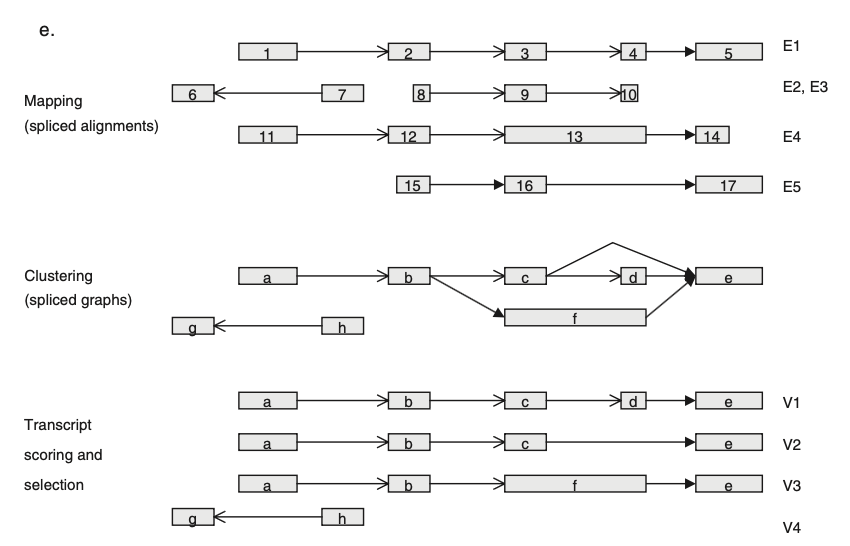
\includegraphics[width=0.7\textwidth]{splice_graph_figure_2e_florea.png}
\caption{EST sequences from the 5' and 3' ends of the gene are compared to identify compatible overlaps and then assembled into consensus sequences (TC1, TC2) representing putative splice variants. Spliced alignments of cDNAs on the genome (E1-E5) are clustered along the genomic axis and consolidated into splice graphs. Vertices in the splice graph represent exons (a-h), arcs are introns connecting the exons consistently with the cDNA evidence, and a branching in the graph signals an alternative splicing event. Splice variants (V1-V4) are read from the graph as paths from a source vertex (with no 'in' arc) to a sink vertex (with no 'out' arc). Adapted from Florea (2005).}
\label{fig:splice_graph}
\end{figure}

\subsubsection{Regulatory Element Identification}

Several computational approaches have been developed to identify cis-regulatory elements that control alternative splicing ([2], pp. 63-65):

\textbf{Consensus sequences} represent simple motif models that use IUPAC codes to specify which nucleotides are allowed at each position in a regulatory sequence ([2], p. 63). However, this approach can only indicate nucleotide permissibility and cannot quantify the relative preference for specific nucleotides at each position.

\textbf{Position Weight Matrices (PWMs)} provide more sophisticated modeling by capturing the relative frequency and preference for each nucleotide at every position within a regulatory motif ([2], p. 64). PWMs are constructed from experimentally identified binding sites and provide quantitative scoring systems where higher scores indicate stronger matches to the consensus motif. For example, PWMs for important splicing factors like SF2/ASF, SC35, SRp40, and SRp55 have been experimentally derived and validated.

\textbf{Statistical k-mer analysis} employs computational approaches to identify short DNA sequences (typically 6-8 nucleotides) that appear with statistically significant over-representation in specific genomic contexts ([2], p. 64). For instance, researchers compare hexamer frequencies in exons versus introns, or in weakly spliced exons versus strongly spliced ones, to identify potential enhancer or silencer elements based on their enrichment patterns.

\textbf{Motif discovery algorithms} like MEME and Gibbs sampling use unsupervised machine learning approaches to identify common sequence patterns in sets of related sequences without prior knowledge of regulatory elements ([2], p. 65). While these methods can discover novel motifs, they may have limited predictive power when applied to large, heterogeneous sequence sets with weak or complex regulatory signals.

\textbf{Comparative genomics} leverages evolutionary conservation analysis to identify functionally important regulatory sequences by comparing orthologous sequences between species ([2], p. 65). This approach is based on the principle that sequences under functional constraint will be preferentially conserved during evolution. Studies have demonstrated that intronic sequences flanking alternatively spliced exons show stronger evolutionary conservation than those around constitutive exons, indicating the presence of important regulatory elements.

\section{Evaluation}

\subsection{Effectiveness of Integrative Experimental Approaches}

The integrative methodology developed by Liu et al. (2017) demonstrates several significant strengths in quantitatively linking splicing changes to proteomic outcomes.

\subsubsection{Quantitative Validation of Splicing Impact}

The approach successfully provided quantitative evidence for specific relationships between splicing events and protein abundance:

\textbf{Intron retention correlation}: The method consistently demonstrated that intron retention events are associated with decreased protein abundance ([1], p. 1237). Introns are the non-coding segments that are normally removed during RNA processing. When introns are unexpectedly retained (kept in) the final mRNA, this consistently leads to less protein being made. This occurs because these faulty mRNAs might get stuck in the nucleus (unable to reach the protein-making machinery) or get destroyed by the cell's quality control system called nonsense-mediated decay (NMD), which cleans up potentially problematic messages.

\begin{figure}[H]
\centering
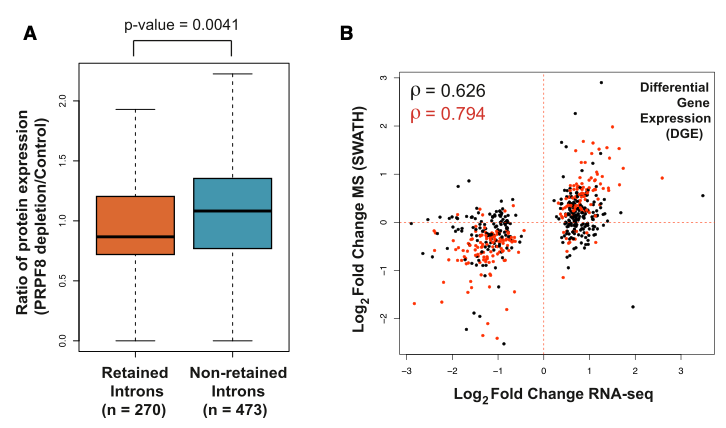
\includegraphics[width=0.5\textwidth]{intron_retention_figure_6_liu.png}
\caption{Intron retention reduces protein levels compared to genes without retained introns. Adapted from Liu et al. (2017).}
\label{fig:intron_retention}
\end{figure}

\textbf{Proportional abundance changes}: Changes in differential transcript usage and differential gene expression produced protein abundance changes proportionate to transcript levels ([1], p. 1238), validating the dominant role of mRNA abundance in determining protein levels under splicing perturbation conditions.

\textbf{Functional validation through isoform switches}: The detailed analysis of lamin-associated polypeptide (LAP2) isoform switching provided compelling evidence for functional consequences ([1], p. 1235). This protein serves as an excellent example because its different isoforms have been well-characterized and do very different jobs in the cell. After PRPF8 depletion, the dominant LAP2 isoform switched from LAP2b to LAP2a ([1], p. 1235). Essentially, the cell switched from making mostly the "b" version to mostly the "a" version. Functionally, \textbf{LAP2b sits at the nuclear lamina} (the inner edge of the nucleus) and acts as a repressor, keeping certain genes quiet, including important targets of p53 and NF-$\kappa$B - key regulators of cell growth, stress response, and inflammation ([1], p. 1235). In contrast, \textbf{LAP2a is found throughout the nuclear interior} and is involved in the structural organization of the nucleus, doing a different job in a different location ([1], p. 1235). The isoform switch led to altered LAP2 localization and \textbf{de-repression of p53 and NF-$\kappa$B transcriptional targets} ([1], p. 1237). In simple terms, since LAP2b (the repressor) was reduced and LAP2a took over, the brakes came off those target genes, which became more active, demonstrating clear biological significance.

\subsubsection{Technical Performance Metrics}

The SWATH-MS approach showed excellent technical performance, demonstrating high reproducibility across biological replicates, comprehensive coverage with 14,695 quantified peptides ([1], p. 1230), successful integration with RNA-seq data through the major transcript strategy, and validation of key findings through targeted SRM analysis.

\subsubsection{Limitations and Challenges}

Despite its successes, the approach faces several limitations:

\textbf{Peptide assignment ambiguity}: Many peptides can theoretically arise from multiple transcript isoforms, requiring strategic decisions about data analysis that may lose some information.

\textbf{Coverage limitations}: Not all proteins or isoforms are equally detectable by mass spectrometry, potentially biasing results toward abundant or easily ionizable peptides.

\textbf{Perturbation model constraints}: The PRPF8 depletion model, while informative, may not fully represent the diversity of splicing perturbations encountered in disease states.

\subsection{Assessment of Bioinformatics Methods}

The bioinformatics approaches surveyed by Florea (2005) show varying degrees of effectiveness depending on the specific application and available data.

\subsubsection{Strengths of Current Methods}

\textbf{Splice graph modeling} represents a major conceptual advance, providing a systematic framework for representing and analyzing all possible splicing patterns within a gene. This approach enables comprehensive enumeration of transcript candidates and facilitates comparative analysis across different conditions.

\textbf{Genome-based approaches} have largely resolved issues with contamination and sequencing errors that plagued earlier gene index methods by using high-quality genome sequences as reference frameworks.

\textbf{Comparative genomics approaches} have proven particularly powerful for identifying functionally important regulatory elements, as demonstrated by the observation that intronic sequences flanking alternatively spliced exons show stronger evolutionary conservation than those around constitutive exons.

\textbf{PWM-based motif modeling} provides quantitative frameworks for predicting regulatory element strength, moving beyond simple binary presence/absence determinations.

\subsubsection{Ongoing Challenges}

\textbf{Biological relevance assessment}: A persistent challenge is distinguishing computationally predicted splice variants that represent real biological isoforms from artificial constructs generated by analysis algorithms. While methods like ECgene attempt to score candidates based on evidence strength, this remains an active area of development.

\textbf{Regulatory element prediction}: Despite advances in motif discovery and PWM modeling, predicting the functional impact of regulatory elements remains challenging, particularly for weak regulatory signals or complex combinatorial interactions between multiple elements.

\textbf{Scalability and computational costs}: Many approaches, particularly gene index methods, face significant computational challenges when applied to large-scale datasets, limiting their practical applicability.

\textbf{Limited predictive power}: While current methods excel at cataloging known splicing events, their ability to predict novel splicing patterns or regulatory relationships remains limited, particularly when applied to diverse sequence sets with weak signals.

\subsection{Comparative Assessment}

When evaluated together, the experimental and bioinformatics approaches show complementary strengths:

\textbf{Experimental validation}: The integrative experimental approach provides essential quantitative validation of computational predictions, bridging the gap between transcriptomic observations and functional proteomic outcomes.

\textbf{Comprehensive coverage}: Bioinformatics methods enable genome-wide analysis and systematic cataloging that would be impractical through purely experimental approaches.

\textbf{Hypothesis generation}: Computational methods effectively generate testable hypotheses about splicing regulation and functional significance that can be validated through targeted experimental approaches.

\textbf{Clinical translation potential}: The combination of computational prediction and experimental validation provides a robust foundation for clinical applications, enabling both discovery of disease-relevant splicing events and quantitative assessment of therapeutic interventions.

\section{Conclusion}

The analysis of these complementary approaches to studying alternative splicing reveals significant advances in our ability to understand and quantify the relationship between splicing patterns and proteome composition. The integrative experimental methodology developed by Liu et al. (2017) represents a breakthrough in directly measuring how splicing perturbations translate into functional proteomic changes, while the bioinformatics frameworks surveyed by Florea (2005) provide the computational foundation for systematic analysis of splicing diversity and regulation.

The key findings demonstrate that alternative splicing serves as a critical regulatory mechanism that functionally tunes the human proteome. The quantitative evidence shows that changes in isoform usage manifest as measurable protein abundance changes, with clear relationships between specific splicing events and their proteomic consequences. The successful demonstration of functional significance through examples like LAP2 isoform switching validates alternative splicing as a mechanism for achieving biological complexity from limited genetic resources.

Most importantly, these methodological advances establish a foundation for translating splicing research into therapeutic applications ([1], p. 1238). The ability to quantitatively measure splicing-proteome relationships opens new possibilities for \textbf{therapeutic manipulation of splicing}, enabling the design of therapies that correct faulty splicing patterns or selectively promote beneficial isoforms over harmful ones. This foundation also supports \textbf{diagnostic tool development} through identification of specific isoform signatures that characterize disease states or predict treatment responses. Additionally, the approach enables \textbf{personalized medicine applications} that target specific splicing events driving disease in individual patients, moving beyond one-size-fits-all treatments to precision therapies tailored to each patient's unique splicing profile. Finally, these advances allow for \textbf{fine-tuning the proteome for health} by developing strategies to therapeutically modulate the cellular protein landscape through controlled alternative splicing patterns, potentially correcting disease-associated protein imbalances.

The convergence of experimental quantification and computational prediction provides the necessary tools to move from cataloging splicing diversity to actively manipulating it for therapeutic benefit. As many human diseases involve splicing defects, this represents an exciting frontier in precision medicine where the detailed understanding of splicing mechanisms can be translated into targeted interventions for improved patient outcomes.

Future research directions should focus on expanding these integrative approaches to disease-relevant systems, developing more sophisticated computational models that better predict functional significance, and translating these insights into clinical applications for the benefit of patients with splicing-related disorders.

\section{References}

[1] Liu, Y., Gonzàlez-Porta, M., Santos, S., et al. (2017). Impact of Alternative Splicing on the Human Proteome. \textit{Cell Reports}, 20, 1229–1241.

[2] Florea, L. (2005). Bioinformatics of alternative splicing and its regulation. \textit{Briefings in Bioinformatics}, 7(1), 55-65.

[3] International Human Genome Sequencing Consortium. (2004). Finishing the euchromatic sequence of the human genome. \textit{Nature}, 431, 931-945.

[4] Mott R. EST\_GENOME: a program to align spliced DNA sequences to unspliced genomic DNA. \textit{Comput Appl Biosci} 1997;3:477–78.

[5] Florea L, Hartzell G, Zhang Z, et al. A computer program for aligning a cDNA sequence with a genomic DNA sequence. \textit{Genome Res} 1998;8:967–74.

[6] Wheelan SJ, Church DM, Ostell JM. Spidey: a tool for mRNA-to-genomic alignments. \textit{Genome Res} 2001;11:1952–57.

[7] Usuka J, Zhu W, Brendel V. Optimal spliced alignment of homologous cDNA to a genomic DNA template. \textit{Bioinformatics} 2000;16:203–11.

[8] Kent WJ. BLAT–the BLAST-like alignment tool. \textit{Genome Res} 2002;12:656–64.

[9] Florea L, Di Francesco V, Miller J, et al. Gene and alternative splicing annotation with AIR. \textit{Genome Res} 2005;15:54–66.

[10] Lee BT, Tan TW, Ranganathan S. MGAlignIt: a web service for the alignment of mRNA/EST and genomic sequences. \textit{Nucleic Acids Res} 2003;31:3533–36.

[11] Wu TD, Watanabe CK. GMAP: a genomic mapping and alignment program for mRNA and EST sequences. \textit{Bioinformatics} 2005;21:59–75.

\end{document} 